\chapter{研究设计与数据概览}
%%====================================================================

本章是两项实证研究的共同基础，集中呈现研究框架、数据来源与融合流程、
方法论选择逻辑及伦理考量。将上述共性内容整合于独立章节，
一方面避免两项研究各自重复叙述而削弱论文的整体感，
另一方面也便于读者在进入具体实证分析之前形成全局认知。

\section{研究框架}

本文围绕“比特币开源社区开发者活动的影响因素”这一核心命题展开，
设计了两项实证研究——二者在研究对象、数据基础和时间窗口上相互衔接，
在研究问题和方法论上彼此互补。
图~\ref{fig:overall-framework} 展示了两项研究在整体逻辑中的定位与关联。

\begin{figure}[htbp]
    \centering
    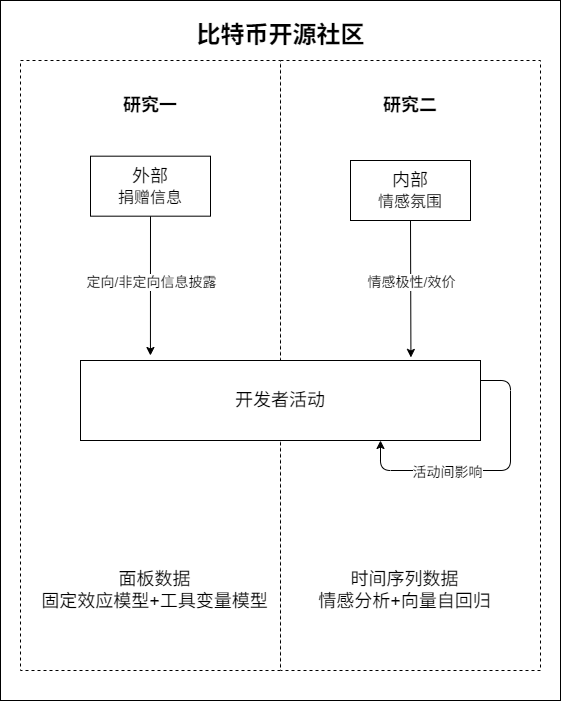
\includegraphics[width=0.52\textwidth]{figures/overall_framework.png}
    \caption{研究框架}
    \label{fig:overall-framework}
\end{figure}

研究一以个体开发者为分析单元，考察外部非盈利基金会（Bitcoin Brink）
两类捐赠信息披露事件对开发者活动水平的因果影响。
该研究设计的关键之处在于：剔除实际受资助的8名开发者后，
分析对象被限定为未直接受益于捐款的1,610名开发者，
由此将信息效应与货币效应干净地分离开来。
在估计策略上，固定效应模型控制开发者个体特征与时间共同趋势，以识别信息披露的净效应；
工具变量方法则进一步应对捐款金额与社区活动之间可能存在的反向因果。

研究二转向社区整体层面，考察比特币 Issue 讨论区中提取的情感极性指标
在时间维度上如何影响代码活动与讨论活动，
并探究两类开发活动之间是否存在动态替代关系。
该研究将情感、代码活动和讨论活动三个变量均视为内生变量，
借助向量自回归模型捕捉多变量时间序列系统内的动态反馈机制，
再通过格兰杰因果检验与脉冲响应函数对影响路径加以识别和可视化。

两项研究的分析对象有所不同——研究一关注个体层面的动机响应，
研究二关注社区层面的集体动态——但共享同一时间窗口（2022—2023年）、
同一组核心活动变量（PE、CE、DE、CCE、PRE、PRRE、PRRCE、ISE、ICE）及同一底层数据来源（GH Archive）。
“同一情境、互补视角、多层分析”的设计思路，使两项研究得以从不同维度共同支撑
“信息层面因素深刻影响开发者行为”的核心论点\cite{hu2025license}。

\section{数据来源总览与融合流程}

\subsection{全部数据源汇总}

本研究共整合六类数据源，分别覆盖开发者行为、信息披露事件、
市场环境与社会关注度等维度。
表~\ref{tab:data-overview} 汇总了各数据源的基本信息。

\begin{table}[htbp]
    \centering
    \small
    \caption{全部数据来源汇总}
    \label{tab:data-overview}
    \begin{tabularx}{\textwidth}{p{3.2cm}Xp{3.2cm}p{3.2cm}}
        \toprule
        数据类型 & 数据源与采集方法 & 时间粒度 & 用途 \\
        \midrule
        GitHub 开发活动
            & GH Archive（gharchive.org）；BigQuery 批量下载 & 事件级→周级聚合
            & 研究一、二因变量 \\
        非定向披露信息
            & X 平台 @bitcoinbrink 历史推文；X API v2 & 事件级
            & 研究一核心自变量 \\
        定向披露信息
            & brink.dev 官网存档；手工整理 + Wayback Machine
            & 事件级
            & 研究一核心自变量 \\
        Bitcoin 市场数据
            & Yahoo Finance；yfinance API & 日级→周级
            & 研究一控制变量 \\
        Google Trends 搜索指数 & Google Trends；pytrends 接口，美国地区
            & 周级
            & 研究一工具变量 \\
        Issue 评论文本
            & GH Archive + GitHub REST API；关键词过滤 + 分页拉取 & 评论级→周级聚合
            & 研究二情感分析 \\
        \bottomrule
    \end{tabularx}
\end{table}

GH Archive\footnote{GH Archive 项目主页：\url{https://www.gharchive.org}。} 由 Ilya Grigorik 维护，是一项 GitHub 事件归档服务。
该服务自2011年起以小时为粒度持续记录 GitHub 平台上的全量公开事件，
并经由 Google BigQuery\footnote{Google BigQuery 是 Google Cloud 提供的无服务器、高扩展性的数据仓库服务，支持使用标准 SQL 对 PB 级数据集进行快速查询。} 开放免费的大规模查询接口。
本研究从中提取了 \texttt{bitcoin/bitcoin} 仓库的九类事件：
PushEvent（PE）、CreateEvent（CE）、DeleteEvent（DE）、CommitCommentEvent（CCE）、
PullRequestEvent（PRE）、PullRequestReviewEvent（PRRE）、
PullRequestReviewCommentEvent（PRRCE）、IssuesEvent（ISE）和 IssueCommentEvent（ICE），
覆盖代码提交、分支管理、代码注释、合并请求、代码审查与议题讨论等核心活动类型。

Google Trends 数据经 pytrends Python 接口采集，
以关键词“Bitcoin Brink”在美国地区的周搜索量指数（0—100标准化分值）
度量公众对 Brink 基金会的关注程度。
之所以选取美国地区，是因为比特币核心开发者及主要捐赠方多集中于美国，
该地区的搜索热度对捐款规模具有较强的预测能力，
在第一阶段回归中与内生变量的相关性也更为显著。

\subsection{数据清洗与匹配流程}

六类数据源在格式、粒度和标识符体系上各有差异，
须经系统清洗与匹配方可形成可供分析的面板数据集。
本研究按以下五个步骤依序完成数据整合：

第一步，开发者 ID 统一化与机器人过滤。
GH Archive 事件以 actor\_id（数字型）与 actor\_login（字符串型）
双字段标记行为主体。本研究对两者建立双向映射，
确保同一开发者在不同时期使用不同账号名时不会被误计为多人。
机器人账号则依据账号名称正则规则予以剔除，
筛除对象包括名称含有“bot”“[bot]”“robot”等标记词的账号，
以及 GitHub Actions、Dependabot 等平台内建自动化账号。
该步骤共识别并移除约30个机器人账号。

第二步，时间对齐。
全部数据源统一采用协调世界时（UTC）作为时区基准，
以 ISO 8601 周标准（周一起始）为时间颗粒，
将事件时间戳逐一转换为 ISO 周标识符（格式：YYYY-WXX），
使六类数据能够在相同时间键上完成关联合并。

第三步，样本筛选。
保留2022年1月（2022-W01）至2023年12月（2023-W52）共105个 ISO 周内
在 bitcoin/bitcoin 主仓库至少有一次活动记录的开发者，
并进一步剔除观测期内实际获得 Bitcoin Brink 全职资助的4名开发者。
如此处理后，研究一最终样本中的所有个体均未因捐赠直接受益，
回归系数所反映的即为信息披露的纯信息效应。
最终样本涵盖1,610名开发者，约169,785个开发者-周观测单元。

第四步，披露事件标记。
Brink 在 X 平台发布的非定向披露公告日期与官方网站发布的定向披露公告日期，
被分别精确映射至对应 ISO 周，据此生成两个变量：非定向披露金额变量
（披露金额取自然对数，无披露周取0）与定向披露虚拟变量
（定向披露公布后各周取1，公布前取0）。

第五步，情感聚合与评分。
将 GH Archive 中 bitcoin/bitcoin 主仓库 Issue 区的评论文本按周聚合为整周文本块，
随后由大型语言模型对各周文本进行一次性情感评分，
得到每周的情感极性得分（取值区间 $[1, 9]$，5 为中性基准；
高于 5 表明正面情感占主导，低于 5 则表明负面情感占主导）。
该得分作为当周社区整体情感极性指标，供研究二 VAR 分析使用。

\section{方法论总述}

\subsection{两种方法的问题定位}

两项研究面临的计量问题性质各异，故采用了互补的方法论路径。
表~\ref{tab:method-comparison} 对比说明了两种方法的核心特征及适用场景。

\begin{table}[htbp]
    \centering
    \caption{两种方法的问题定位与适用场景对比}
    \label{tab:method-comparison}
    \begin{tabularx}{\textwidth}{lXXX}
        \toprule
        方法 & 适用问题类型 & 应用于 & 核心解决的挑战 \\
        \midrule
        面板固定效应 + 2SLS
            & 识别外生冲击对个体的因果效应
            & 研究一
            & 个体异质性 + 内生性（反向因果）\\
        向量自回归
            & 刻画多变量系统的动态互动机制
            & 研究二
            & 双向因果（三变量均内生，无先验主从关系）\\
        \bottomrule
    \end{tabularx}
\end{table}

研究一的核心任务在于识别捐赠信息披露对开发者活动的因果效应，
而该场景面临两类典型内生性威胁。
其一为个体异质性——不同开发者在技能水平、内在动机和活跃程度上
存在持续性的横截面差异，不加控制便会产生遗漏变量偏误；
其二为反向因果——社区整体的活跃程度可能影响外部捐赠者的捐赠意愿，
进而左右 Brink 的披露频率与金额，致使因果方向混淆。
面板固定效应模型可有效处理第一类威胁，
工具变量方法则进一步应对第二类威胁，
二者结合构成识别纯信息效应的核心策略。

研究二的核心任务则是刻画情感、代码活动与讨论活动三个变量间的动态反馈机制。
有别于研究一，研究二中并不存在明确的“外生冲击者”与“被冲击者”之分：
情感可能影响活动，活动亦可能反过来塑造情感；代码活动与讨论活动之间同样如此。
向量自回归模型将三个变量均纳入内生系统，
以联立方程组同时捕捉各方向的动态反馈关系，
无需对因果方向施加不可检验的先验假定\cite{sims1980macroeconomics}。
Cornell 等人（2025）在加密货币市场的研究中即采用了类似 VAR 框架，
印证了该方法在刻画加密货币生态内多变量因果网络时的适用性\cite{cornell2025vector}。

\subsection{固定效应模型的识别逻辑}

固定效应模型在基准回归方程中引入两维固定效应，以控制两类系统性偏误。
开发者个体固定效应 $u_i$ 吸收所有不随时间变化的个体特征：
编程技能水平、在比特币社区的参与年限、初始内在动机偏好，
以及其他可能同时影响活动水平与披露信号响应强度的稳定属性。
时间固定效应 $\theta_t$ 则吸收全体开发者在同一周共同面临的宏观趋势——
比特币价格的长期周期、加密货币监管政策的阶段性变动、
比特币生态整体的技术演进节奏，乃至各周内对所有开发者产生同质影响的其他外部因素。

双维固定效应控制下，核心系数 $\beta_1$ 所捕捉的
是”排除开发者个体差异与全局时间趋势后，
捐赠披露信息变动对个体开发者活动水平的净效应”——亦即信息披露的纯增量影响。
在此基础上，工具变量方法引入“Bitcoin Brink” Google Trends 搜索量指数
作为捐款金额的工具变量，以进一步处理捐款金额变量自身的内生性。
有效工具变量须满足两个条件。
相关性条件要求工具变量与内生变量显著相关：本研究中公众 Google 搜索热度
与 Brink 所获捐款金额呈正向相关，
第一阶段回归 F 统计量超过10这一传统强工具变量门槛，相关性得以确认。
排他性条件要求工具变量仅经由内生变量影响因变量，不存在直接路径。
公众在 Google 上搜索“Bitcoin Brink”的行为，本质上反映的是社会层面对该机构的信息兴趣，
并不直接决定比特币 GitHub 上某位特定开发者当周的活动行为，在理论上满足排他性约束。

\subsection{VAR 模型的识别逻辑}

向量自回归模型将情感（$\text{Sentiment}_t$）、代码活动（$\text{CodeActivity}_t$）
与讨论活动（$\text{DiscussActivity}_t$）三个变量组成系统向量 $\mathbf{y}_t$，
以联立方程形式捕捉变量间的动态反馈：

\begin{equation}
\label{eq:var-overview}
\mathbf{y}_t = \mathbf{c} + \sum_{k=1}^{p} \mathbf{A}_k \mathbf{y}_{t-k} + \boldsymbol{\varepsilon}_t
\end{equation}

其中 $\mathbf{A}_k$ 为第 $k$ 期的系数矩阵，$\boldsymbol{\varepsilon}_t$ 为白噪声残差向量。
滞后阶数 $p$ 依 AIC/BIC 信息准则确定，
优先取使信息准则最小化的较低阶数，
从而在模型拟合充分性与过拟合风险之间求得平衡。

格兰杰因果检验基于受限与无约束 VAR 模型的似然比统计量，
在统计层面判断“变量 X 的历史值有助于预测变量 Y 的当前值”——
若有助于预测，即称 X 格兰杰引起Y。
需指出，格兰杰因果所确立的是统计层面的预测能力判据，
并不等同于结构性因果关系；不过，结合本研究的理论预期与情境合理性，
它可作为动态影响路径存在的重要证据。

脉冲响应函数采用 Cholesky 分解对冲击施以正交化处理，
排列顺序设定为“情感 → 代码活动 → 讨论活动”。
该顺序的理论依据如下：情感状态作为信息环境的即时反映，
在逻辑上先于行为响应而形成；代码活动因时间成本较高，
对情感信号的响应相对迟缓；
讨论活动则参与门槛较低，对外部信号可作出更即时的响应，
故在三者的因果排序中居于末位。方差分解进一步量化各变量
对系统中其他变量预测误差方差的解释占比，
有助于评判各变量在整体动态系统中的相对重要性。

\section{伦理考量}

\subsection{数据公开性与合规性}

本研究使用的全部数据均取自公开渠道，研究性使用符合相关平台服务条款及
学术研究惯例。具体而言，GH Archive 作为 GitHub 对外开放的事件归档服务，
采用 CC BY 4.0 授权协议，允许研究性使用与再发布。
X 平台 @bitcoinbrink 账号的推文系公开账号主动发布的信息，
不涉及私信或受访问控制的内容。
Brink 官网公布的受资助开发者名单属于非盈利组织主动向社会公开的资助记录——
系自愿信息披露行为，本研究对其进行学术性整理和引用具有充分合理性。
Google Trends 与 Yahoo Finance 所提供的数据均为面向公众的聚合统计数据，
不含个人识别信息，研究使用不存在合规障碍。

\subsection{开发者隐私保护}

数据处理与结果呈现环节均充分顾及开发者隐私保护。
分析所用开发者标识符为 GitHub 平台的公开用户名（actor\_login）
及数字型 ID（actor\_id），不涉及私人联系方式、地理位置信息或
任何未经公开披露的个人数据。
统计结果的汇报一律以聚合形式呈现，
回归系数反映的是样本整体的平均处理效应，
不对特定开发者的个体行为作点名式描述。
文中涉及的受资助开发者姓名
均来自 Brink 官方网站已公开发布的信息，未超出既有公开范围。

\subsection{数据安全与可复现性}

原始数据存储于本地加密硬盘及受访问控制的服务器环境，
研究过程中不对原始数据作外部分发或共享。
数据分析所用 Python 脚本与 Stata 代码将于论文答辩完成后，
经匿名化处理后通过 GitHub 代码仓库对外开放，以支持可复现性审查。
该代码仓库不包含任何可识别作者信息的内容，
以满足同行评审的匿名性要求。


